\chapter{Adversarial Derivations}
Here we look at the problem of crafting adversarial derivations for text.  Our goal is to alter a text sample in a small way which is not immediately noticeable to a reader, and yet causes a classifier to misclassify a particular sample.  This problem was originally studied in the context of image classification with convolutional neural networks.  Here we consider a few different kinds of adversarial derivations/examples.

\section{Adversarial Examples} 
Adversarial examples were originally defined in the domain of image classification in the form of a constrained optimization problem.  The following definition is similar to \cite{cs14}.  We take images to be vectors in $\mathbb{R}$, and $S$ is a finite set of classes, so that a classifier $f:\mathbb{R}\rightarrow S$ assigns each image a unique class.

\begin{definition}
An adversarial derivation, $x + r \in \mathbb{R}^m$, of an image, $x \in \mathbb{R}^m$ for a classifier, $f$, is a solution to the following optimization problem:
\end{definition}

\noindent
minimize $||r||_2$ subject to:
\begin{enumerate}
\item $f(x + r) \neq f(x)$
\item $x+r \in [0,1]^m$
\end{enumerate}
We may also denote the adversarial derivation as $x^* = x + r$

\noindent
In words, an adversarial derivation is a sample with the minimum distance to a true sample such that it is classified as something different.  We also require that every element stays in the interval $x_n+r_n \in [0,1]$ because actual pixels must remain in some constant bounded interval.

\begin{definition}
A classifier, $f$, over a set, $D$, is a mapping, $f : D\rightarrow \{1,2,\dots,K\} = C$.
\end{definition}

Clearly, this adversarial derivation definition does not translate well to the problem of natural language classification where the domain is not even numeric.  We give a more general  constrained optimization defintion below, which we will adapt to the problem of creating adversarial derivations for text.

\begin{definition}
A distance function, $d$, over a set $S$ is a mapping, $d:S\times S\rightarrow \mathbb{R}$ such that $\forall x,y,z \in S$:
\begin{enumerate}
\itemsep0em
\item $d(x,y) \geq 0$
\item $d(x,y) = 0 \iff x=y$
\item $d(x,y) \leq d(x,z) + d(z,y)$
\end{enumerate}
\end{definition}

\noindent One important example of a distance metric is the discrete metric, given by

\[
\rho(v,v^*) =
\begin{cases}
0 & \text{if $v = v^*$} \\
1 & \text{if $v \neq v^*$} \\
\end{cases}
\]
\noindent
It is also true that if $S$ is a normed linear space, $d(x,y) = ||x-y||$ is a distance metric over that space.

\begin{definition}
Let $d_D$ be a distance function over $D$, and $d_C$ be a distance function over $C$.  Then the point $x^*$ is an adversarial derivation (AD) of $x\in D$ with tolerance $\epsilon > 0$ given by
\begin{equation*}
\begin{aligned}
& \underset{x^*\in D(f)}{\text{min}}
& & d_D(x,x^*) \\
& \text{subject to}
& & d_C(f(x),f(x^*)) > \epsilon
\end{aligned}
\end{equation*}
\end{definition}

\noindent
Note that image classifier would have the domain $[0,1]^m$ and codomain $ \{1,...K\} $ where $K$ is the number of classes.  So the definition of an adversarial derivation for an image classifier is the same as the general definition if we let $\epsilon = 1$, $d_D(x,x^*) = ||x-x^*||^2$, $d_C(y,y^*) = |y-y^*|$.

As long as the function, $f$, has a non-singleton codomain, the constraint is satisfiable for for small enough $\epsilon$.  In the case that the solution does not exist, $\delta = \inf \{d_D(x,x^*) \text{ s.t. } d_C(f(x),f(x^*)) > \epsilon\}$ exists, in which case we may find $\hat{x}$ that is arbitrarily close to $\delta$.  Satisfiability is true from the fact that for any distance metric, $d(y,y^*) > 0$ for $y \neq y^*$.  That all being said, the distance between the sample and the derived sample may be so large that they are easily recognized to be different.  We therefore define a similar problem with very different properties

\begin{definition}
An absolutely adversarial derivation (AAD) of $x$ with similarity $\delta$, difference $\epsilon$, domain metric $d_D$, and codomain metric $d_C$ is given by any solution to the following two constraints.

\begin{equation*}
\begin{aligned}
& & d_D(x,x^*) < \delta\\
& & d_C(f(x),f(x^*)) > \epsilon
\end{aligned}
\end{equation*}
\end{definition}

In this less relaxed version of the problem, a solution may not exist.  In fact, for a given continuous function, $f$, defined on an open domain, and tolerance, $\epsilon$ it is guaranteed that $$\exists \delta > 0 \text{ s.t. } d_C(f(x),f^*(x)) < \epsilon$$ meaning no solution exists.  However, it appeals to a more intuitive concept and allows for the possibility of a model immune to adversarial attacks.  It says that the sample and its absolute adversarial derivation must be sufficiently close and the distance between the model outputs must be sufficiently far.  

It is easy to see that if an AAD exists for a given sample, then any AD is also an AAD.  This means we may solve the more relaxed problem to obtain a valid solution, and so we will work with the more practical objective of creating ADs.

\section{Word Embeddings}\label{sec:word_embeddings}
Consider the common scenario of a text classifier which maps plain text files to one of several classes.  It is common for the plain text to first be processed into a sequence of tokens, which are then each assigned an integer resulting in a sequence of integers.

\begin{definition}
Let $s$ be a sequence of characters.  Let $a_n \in \{0,1,\dots,V\} \forall n \in \{0,1,\dots,N\}$ and $E:s\rightarrow \{a_n\}_{n=1}^{N_s}$.  Then we call $E$ an encoder, $V$ the encoder vocabulary size, and $N_s$ the sample length with respect to $E$.
\end{definition}

In plain words, an encoder maps a string to a sequence of bounded integers.  The sequence is some length which depends on both the encoder and the string.  We assume a fixed encoder, and therefore vocabulary size, $V$.  Since, after encoding, the distance between one word and another is arbitrary, we further translate into a one-hot encoded vector.  That is, the integer $n$ is mapped to a vector where the $n^{th}$ element is $1$ and all others are $0$.  This ensures that all vectors representing words are unit norm and the distance between any two different words is the same.  We denote the set of one-hot encoded vectors of size $V$ as $1_V$.

This simple method of representing words as vectors results in a very high dimension representation of all words in the vocabulary, and thus even a very simple linear model would be very large and difficult to train.  Using the word2vec model discussed in the previous chapter, the dimension of this representation can be significantly reduced, while also encoding information about statistical semantic similarity about each word.

\begin{definition}
Let $f: 1_V \rightarrow \mathbb{R}^D$.  We call $f$ a word embedding and we call $D$ the size of $f$, or embedding size.
\end{definition}

\noindent
Let $W \in M_{D\times V}(\mathbb{R})$.  Then clearly any word embedding, $f$, of size $D$ may be represented as the matrix multiplication $Wv$ $\forall v \in 1_V$.  The matrix $W$ is called the embedding matrix.  This numerical representation of words is extremely useful since we can now apply more general and modern techniques to solving the problem of classification.


\section{Adversarial Text Derivation}
\noindent
Now that we have a clear idea of both the domain and numerical representation of words, we may define an adversarial derivation of textual data in the context of a classification model, $f$.  As per the definition of an adversarial derivation, we need only to define the model tolerance, $\epsilon$, as well as the domain metric, $d_D$ and codomain metric, $d_C$.  We will consider primarily two definitions.

\begin{definition}
Let $\{v_i\}_{i=1}^N$ be the sequence of vectors obtained from a given word embedding and text sample, then a discrete adversrial derivation is defined has having domain metric, $d_D(v,v^*) = \sum_i^N\rho(v_i,v_i^*)$, codomain metric $d_C(f(v),f(v^*)) = \rho(f(v),f(v^*))$, and tolerance $\epsilon = 1$.
\end{definition}

That is, a discrete adversarial derivation $\{v_i^*\}$ of sample $\{v_i\}$ is the sample which changes the least amount of words possible, while changing the classification.  This definition is simple, though it may not yield very good results if solved.  For example, a positive movie review, ``This movie was good'' could easily be changed to a negative review by changing just one word resulting in ``This movie was bad''.  These two samples would obviously have different sentiments if read by a human.

%Clearly the codomain metric, $d_C$ and difference, $\epsilon$ make sense for any defintion in this context, but the domain metric has room for improvement which brings us to the next definition.

%\begin{definition}
%A semantic adversarial derivation is defined as having angular distance as the domain metric and the same difference and codomain metric as a discrete adversarial derivation.
%\end{definition}

%If we minimize this objective, then we would tend to use semantically similar words in substitution.  However, this does not necessarily solve the problem of actual sentiment inversion.  For instance, in our embedding the semantically closest (measured with the $l^2$ norm) word to ``bad'' is ``good.''  This makes sense since they are semantically very similar and would be used in the same contexts, but may result in obvious semantic flips.  We will therefore look to other metrics in an attempt to find better results.



\chapter{Preliminary Results}
\section{Word Embedding Training}
\label{sec:word_emb_results}
We used gradient descent to train a word2vec model with noise contrastive estimation.  All gradients were calculated with the automatic differentiation framework, TensorFlow \cite{ma16}.  The hyperparameters we chose are shown in Table \ref{tab:embedding_hperparameters}.

\begin{table}[h]
\centering
\begin{tabular}{ l | r }
    \hline
    Learning rate & 1.0 \\
    Batch size & 128 \\
    Number of Batches & 100,000 \\
    Embedding size & 128 \\
    Number of skip windows & 8 \\
    Size of skip windows & 4 \\
    Vocabulary size & 10,000 \\
    \hline
\end{tabular}
\caption{Word embedding hyperparameters.}
\label{tab:embedding_hperparameters}
\end{table}

Our corpus was the concatenation of all preprocessed training samples from the training set in the ``Large Movie Review Dataset.'' \cite{am11}  Preprocessing consisted of the steps laid out in Table \ref{tab:preproc}

\begin{table}[h]
\centering
\begin{tabular}{ l | l }
    \hline
    Start & The movie isn't \verb|{<br \><br />}|good, I give it a 1\\
    Convert to lower case & the movie isn't \verb|{<br \><br />}|good, i give it a 1\\
    Remove HTML & the movie isn't \space good, i give it a 1\\
    Expand contractions & the movie is not \space good, i give it a 1\\
    Remove punctuation & the movie is not \space good i give it a 1\\
    Expand numbers & the movie is not \space good i give it a one\\
    Remove extra whitespace & the movie is not good i give it a one\\
    \hline
\end{tabular}
\caption{Preprocessing Algorithm}
\label{tab:preproc}
\end{table}

The processing resulted in a corpus of 5,887,178 words totaling 31,985,233 characters.  Since there are 25,000 training samples, each review is on average about 234 words, and 1279 characters.  Of all 25,000 reviews training reviews, 27 had more than 1024 words.  The word embedding converged to an average noise contrastive loss of about 5.07.   Semantic difference between two words is measured by the angular distance between their embeddings, computed as

$$ \frac{cos^{-1}\left(\frac{v^Tu}{||v||_2||u||_2}\right)}{\pi}$$

\noindent
The eight nearest neighbors for a few common words are shown in table \ref{tab:nearest_words}.  We can see that the first few nearest neighbors are fairly high quality, and would usually make grammatical sense for replacement in a sentence.  The quality of replacement falls off quickly after that however.

\begin{table}[h]
\centering
\begin{tabular}{ | c |  c  c  c  c  c  c  c  c | }
    \hline
    all & but& some& and& UNK& just& also& that& so \\ \hline
    and & UNK& with& but& also& which& simpler& nerd& just \\ \hline
    will & can& would& if& do& could& to& did& you \\ \hline
    of & in& from& with& for& UNK& about& which& that \\ \hline
    her & his& she& him& he& their& UNK& the& india \\ \hline
    she & he& her& him& his& who& UNK& it& that \\ \hline
    most & all& best& films& which& other& UNK& some& only \\ \hline
    one & three& two& zero& five& only& nine& s& UNK \\ \hline
    movie & film& show& story& it& but& really& that& just \\ \hline 
    film & movie& story& show& which& UNK& it& that& but \\ \hline
\end{tabular}
\caption{Some examples of nearest neighbors in embedding space.}
\label{tab:nearest_words}
\end{table}

\section{RNN Training}
\label{sec:rnn_results}
Here we will focus on one particular type of model which has proven very effective in text classification and prediction, a recurrent neural network utilizing long short-term memory (LSTM) units.  Our base model has one layer of LSTM units where the output of each unit is averaged over time followed by a fully connected layer with two outputs, corresponding to the logits of a positive and negative class.  The network's confidence of a given samples class is given by the softmax of both logits.  

The model was trained for 50 epochs over the entire training set with a batch size of 1000 and a maximum unfolding length of 1024, meaning that 27 reviews would be clipped.  The Adam optimizer with exponential step decay factor of 0.8 every 500 batches was used to minimize the model loss, softmax cross entropy.  We used forget gates, peepholes, and output dropout for training.  

We trained fourteen models, varying the number of hidden units and initial learning rates.  The final training and testing accuracies are shown in tables \ref{tab:train_accuracy} and \ref{tab:test_accuracy} respectively.  As expected, increasing the model size always increased the training accuracy, as did increasing the learning rate.  The testing accuracy was less predictable.  Most accuracies were in the neighborhood of 80\%, 30\% greater than the baseline of 50\% random guessing.

\begin{table}
\centering
\begin{tabular}{ |c|c|c|c|c|c|c|}
    \hline
    \multicolumn{7}{|c|}{Number of Hidden Units, Learning Rate = 0.01}\\ \hline
    2 & 4 & 8 & 16 & 32 & 64 & 128 \\ \hline
    0.778 & 0.784 & 0.812 & 0.850 & 0.878 & 0.904 & 0.961 \\ \hline
    \multicolumn{7}{|c|}{Number of Hidden Units, Learning Rate = 0.1}\\ \hline
    2 & 4 & 8 & 16 & 32 & 64 & 128 \\ \hline
    0.827 & 0.853 & 0.895 & 0.965 & 0.975 & 0.997 & 0.990 \\ \hline
\end{tabular}
\caption{Training Accuracy}
\label{tab:train_accuracy}
\end{table}

\begin{table}
\centering
\begin{tabular}{ |c|c|c|c|c|c|c|}
    \hline
    \multicolumn{7}{|c|}{Number of Hidden Units, Learning Rate = 0.01}\\ \hline
    2 & 4 & 8 & 16 & 32 & 64 & 128 \\ \hline
    0.753 & 0.755 & 0.771 & 0.809 & 0.816 & 0.829 & 0.834 \\ \hline
    \multicolumn{7}{|c|}{Number of Hidden Units, Learning Rate = 0.1}\\ \hline
    2 & 4 & 8 & 16 & 32 & 64 & 128 \\ \hline
    0.793 & 0.816 & 0.827 & 0.822 & 0.815 & 0.809 & 0.817 \\ \hline
\end{tabular}
\caption{Testing Accuracy}
\label{tab:test_accuracy}
\end{table}

The average training and test losses of each model are given in figures \ref{fig:train_curve} and \ref{fig:test_curve}.  The spacing on the training curve is finer because the value was sampled every epoch instead of every five epochs as in the case of the testing accuracy.


\begin{figure}
    \centering
    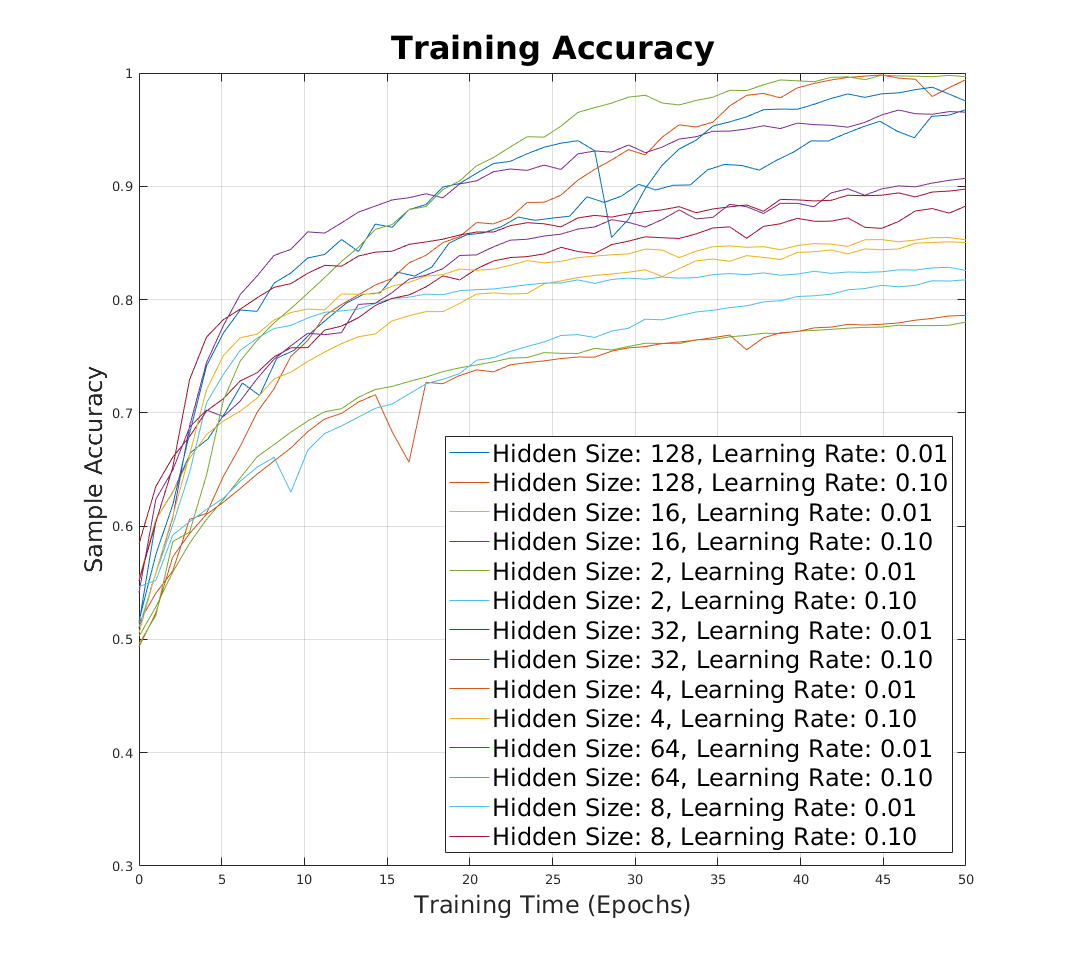
\includegraphics[width=\textwidth]{train_curve.png}
    \caption{Training Accuracy of RNNs}
    \label{fig:test_curve}
\end{figure}

\begin{figure}
    \centering
    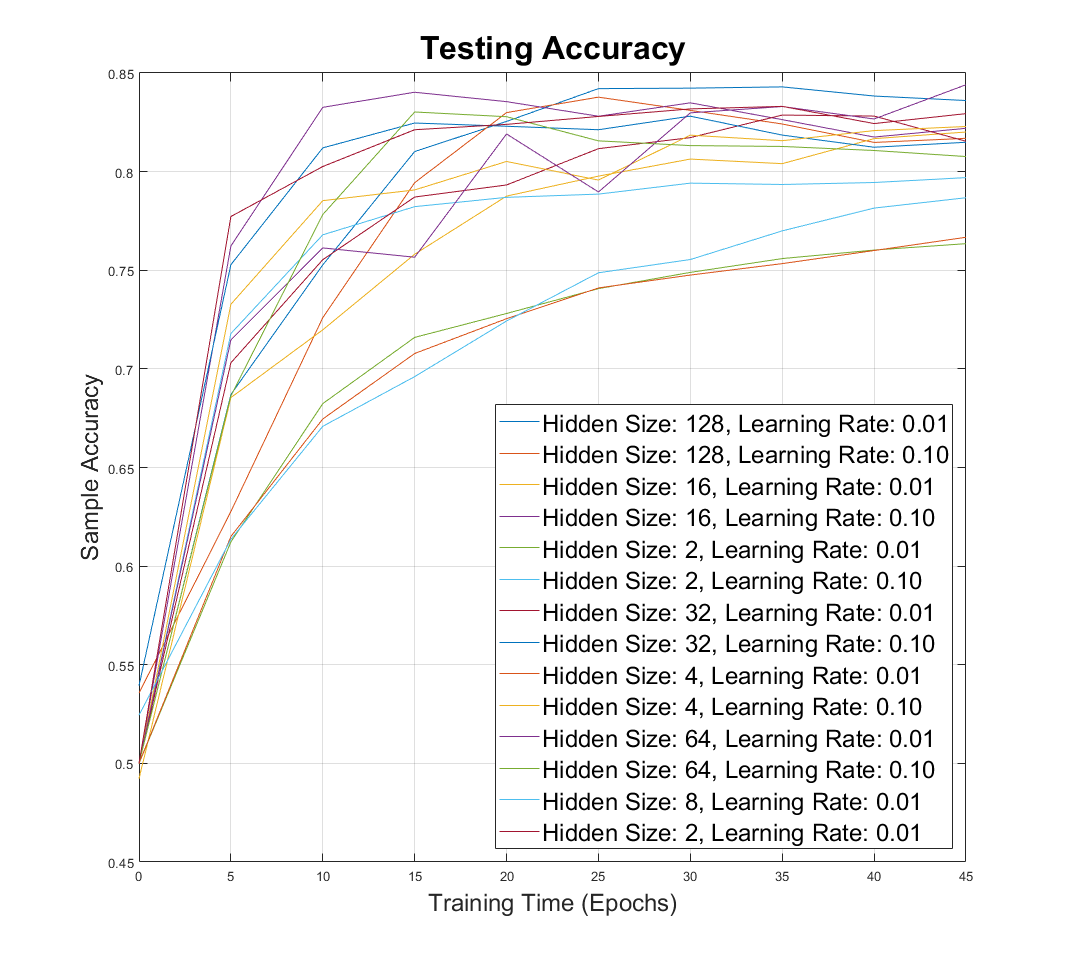
\includegraphics[width=\textwidth]{test_curve.png}
    \caption{Testing Accuracy of RNNs}
    \label{fig:train_curve}
\end{figure}

\section{Stochastic Gradient Analysis}\label{sec:stochastic_gradient_analysis}
\noindent
\begin{definition}
Let the gradient of a model output, $f_i$, with respect to an input vector, $x$ be denoted by $g=\nabla f(x)$.  The total gradient is given by 
\begin{equation}
g_t = \sum_{i=1}^D \nabla f(x)_i
\end{equation}
The gradient norm is given by 
\begin{equation}
g_n = \sqrt{\sum_{i=1}^D |\nabla f(x)_i|^2} = ||\nabla f(x)||_2
\end{equation}
\end{definition}

Both of these measures, along with the gradient itself, are shown for our model as well as a small excerpt of one of the text samples in Figure \ref{fig:saliency}.  We see that the three words with the largest total gradients are ``loved'', ``good'', and ``bad'' which are all sentimental.  First, a differentiable function, $f$, can be locally approximated by
\begin{align}
f(w_j) &\approx f(x_i) + (w_j-x_i)^T\nabla f(x_i) \\
     &= f(x_i) + w_j^T\nabla f(x_i) - x_i\nabla f(x_i) \\
     &= f(x_i) + w_j^Tg - x_i^Tg \label{approx}
\end{align}
Here are considering specificially the affect of replacing the $i^{th}$ input word vector, $x_i$ with the $j^{th}$ embedding word vector, $w_j$ while all other input vectors remain constant.

\begin{definition}

With the above defintions of $x_i$, $w_j$, and $\nabla f(x_i)$, let
\begin{align}
X &= 
\begin{bmatrix}
x_1, x_2, \dots, x_N
\end{bmatrix} \in M_{D\times N}(\mathbb{R})\\
W &= 
\begin{bmatrix}
w_1, w_2, \dots, w_V
\end{bmatrix} \in M_{D\times V}(\mathbb{R})\\
G &= 
\begin{bmatrix}
\nabla f(x_1), \nabla f(x_2), \dots, \nabla f(x_N)
\end{bmatrix} \in M_{D\times N}(\mathbb{R})
\end{align}
\noindent
The approximated perturbation, $f(w_j)-f(x_i)$, of replacing the $i^{th}$ input with the $j^{th}$ embedding word vector is given by 
\begin{align}
    D_{i,j} = (G^TW)_{i,j} - (G^TX)_{i,i}
\end{align}
\noindent
$D$ is called the approximate delta matrix.
\end{definition}
\noindent
For a perfectly linear function, $f$, $D_{i,j} = f(w_j) - f(x_i)$.  We found that for small output differences, the approximation worked fairly well in that a lesser approximate delta tended to produce a lesser actual delta, as seen in figure \ref{fig:dvhat}.  However, the approximation failed almost completely for large differences, as illustrated in figure \ref{fig:outliers}.  This is not surprising given that the model is highly non-linear but it confirms that using the gradient alone is not a reliable technique for discovering adversarial derivations.

\begin{figure}
    \centering
    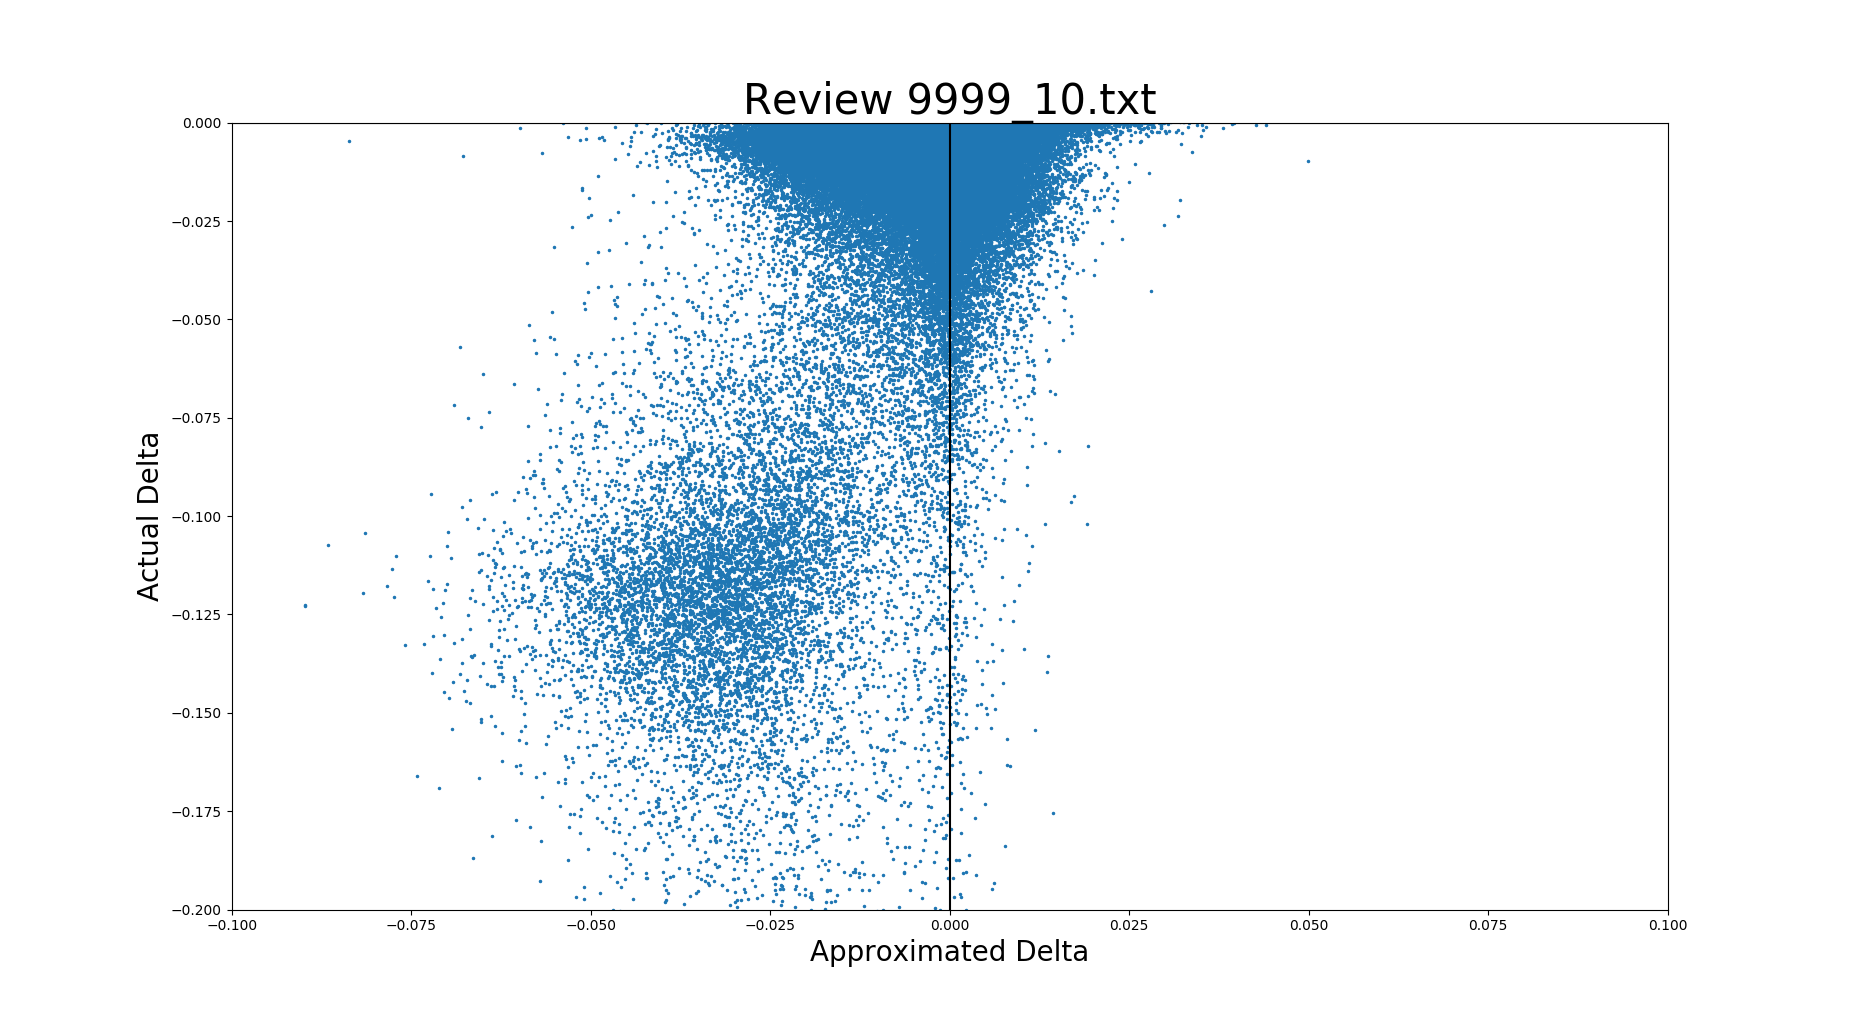
\includegraphics[width=\textwidth]{delta_vs_deltahat.png}
    \caption{Predicted difference in prediction confidence vs. actual difference for sample file 9999\_10.txt}
    \label{fig:dvhat}
\end{figure}

\begin{figure}
\centering
\begin{subfigure}[t]{0.45\textwidth}
  \centering
  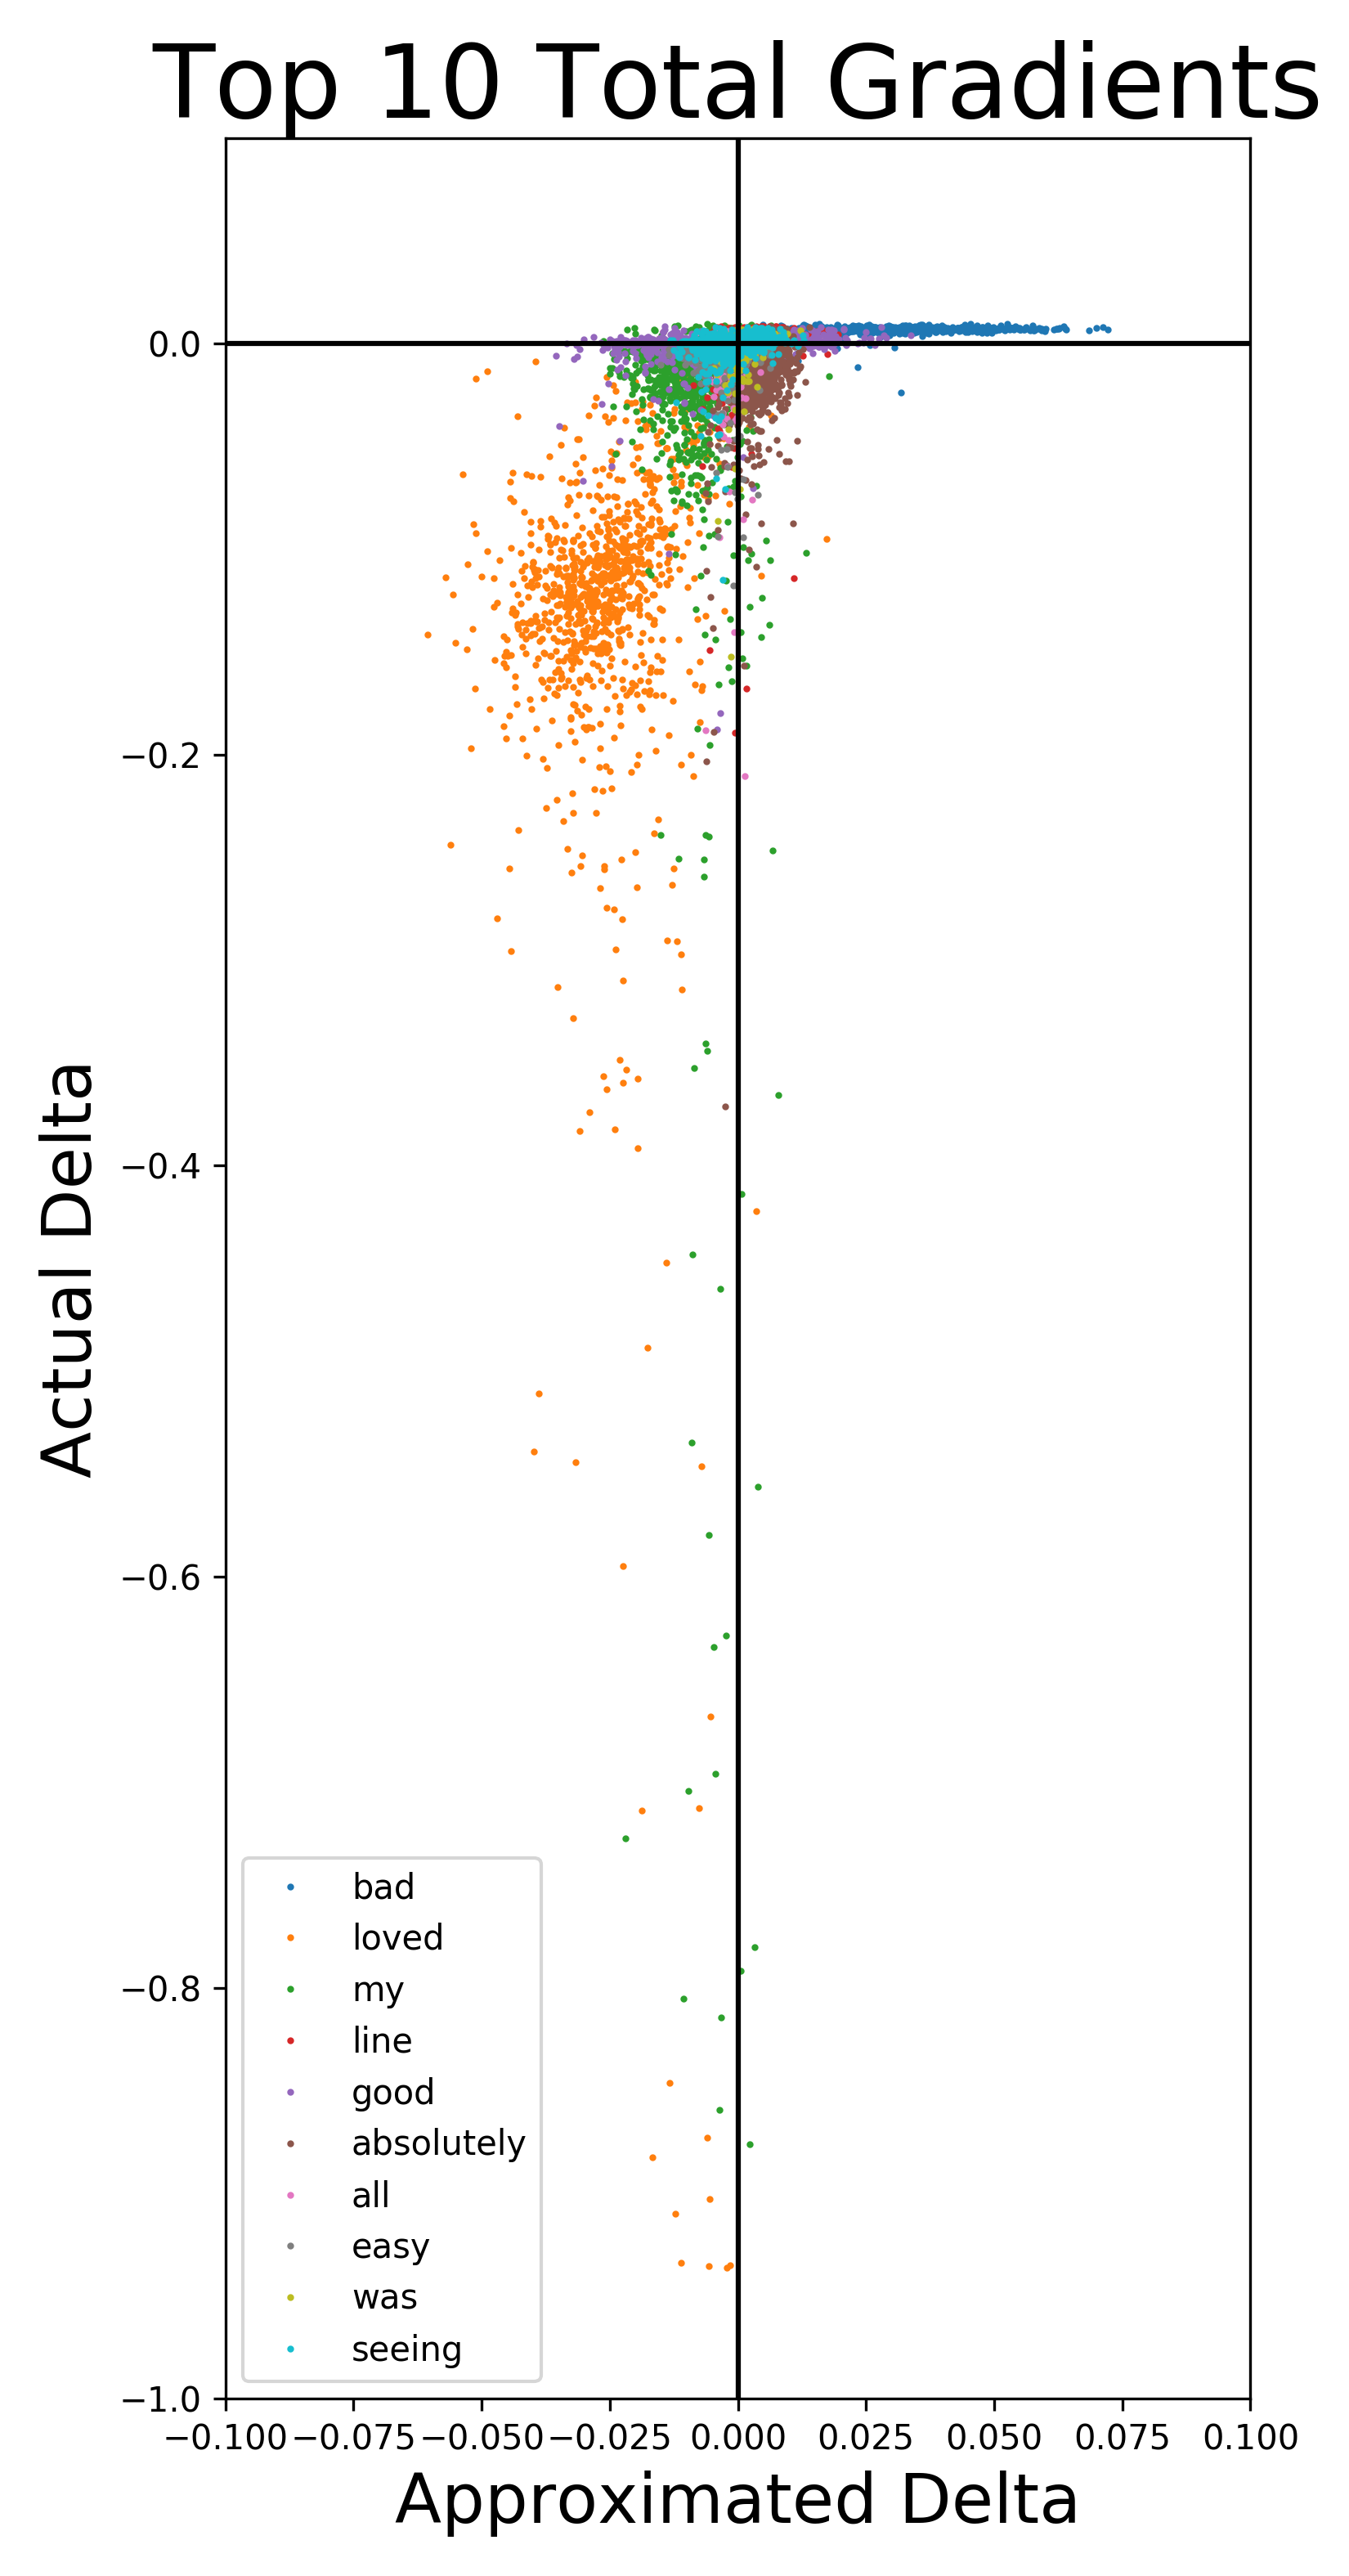
\includegraphics[width=0.9\textwidth]{total_color.png}
  \caption{The words with the top ten largest absolute total gradeints are chosen}
  \label{fig:total_color}
\end{subfigure}\hfill
\begin{subfigure}[t]{0.45\textwidth}
  \centering
  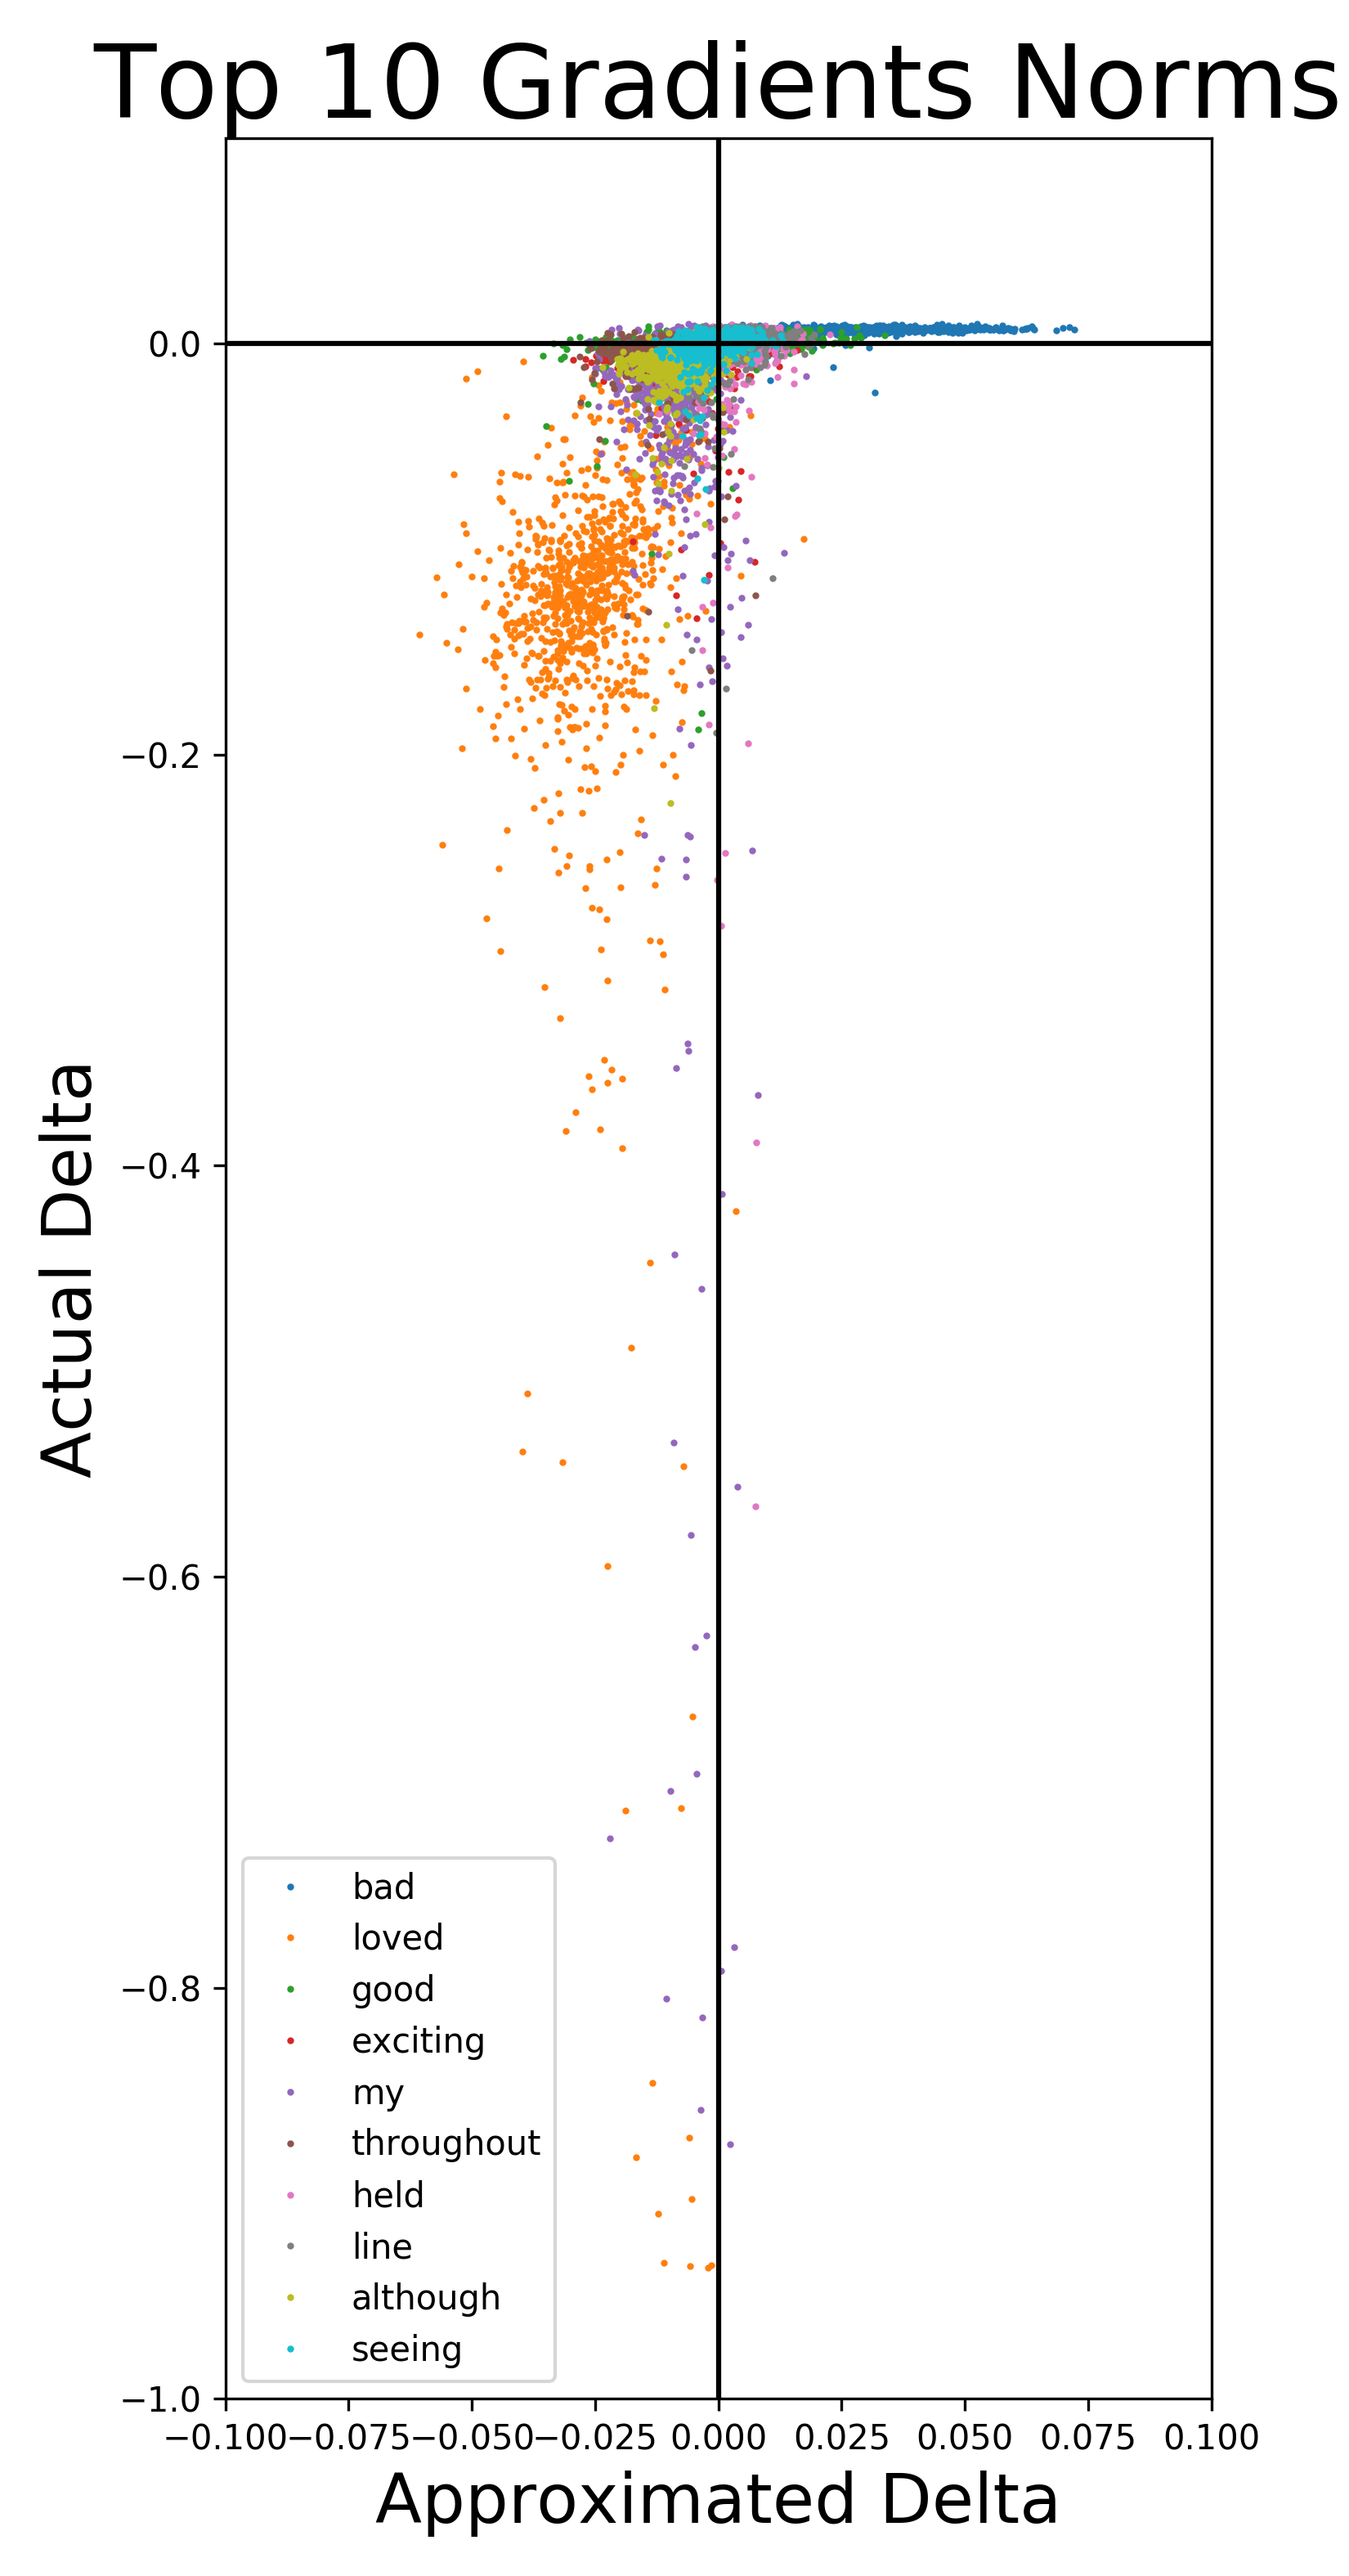
\includegraphics[width=0.9\textwidth]{norm_color.png}
  \caption{The words with the top ten largest gradient norms are chosen}
  \label{fig:norm_color}
\end{subfigure}
\caption{The predicted change in classifier confidence vs. the actual change.  Only the most common 1,000 words are considered in replacement for this example.  The words are listed in the legend in order of decreasing value.}
\label{fig:outliers}
\end{figure}

We see that individual $\hat{D}$ entries are not a good choice for determining which specific words to interchange, but that our measures of gradient may be useful in determining which words are susceptible to attack.  We give motivation with some simplified probabilistic analysis.  Suppose that each of the embedding dimensions is distributed independently and identically across words, with some mean, $\mu$ and variance, $\sigma^2$.  Let $g = \nabla f(x_i)$ for a given word vector, $x_i$ and suppose we replace it with a random word vector, $w_j$.  Recall equation \ref{approx}, we are interested in estimating the term $w_i^Tg = g^Tw_i$ probabilstically since the term $x_i\nabla f(x_i)$ is fixed for a given word.  Let $v=w_i$ and $u=x_i$, then randomly replacing $u$ with another word vector, we have
\begin{equation}
\E{g^Tv} = \E{\sum_{i=1}^D{g_iv_i}} = \sum_{i=1}^D{g_i\E{v_i}} = \mu\sum_{i=1}^D{g_i} = \mu g_t
\end{equation}
\noindent
If we are interested in purposefully altering classification, however, we might be more interested in the expected maximum value of $g^Tv$, that is,
\begin{equation}
Z(g) = \E{\underset{0\leq n\leq V}{\max}\,{g^Tv_n}}
\end{equation}
\noindent
Unfortunately, there is no simple expression which captures this value.  However if we assume that $v_{n,i}$ is distributed normally, we have 
\begin{equation}
Z(g) = \E{\underset{0\leq n\leq V}{\max}\,{g^Tv_n}} = \E{\underset{0\leq n\leq V}{\max}\,{\sum_{i=1}^D{g_i}v_{n,i}}} = \E{\underset{0\leq n\leq V}{\max}\,{p_n}}
\end{equation}
\noindent
where $p_n \sim \mathcal{N}(\mu g_t,\sigma^2 g_n^2)$  There is still no closed form expression for this value, but there is a known \cite{pm07} upper bound:
\begin{align}
Z(g) &\leq \mu g_t + \sigma g_n\sqrt{2\log{V}}\\
\E{\max \hat{D}_{i,*}} &\leq \mu g_t + \sigma g_n\sqrt{2\log{V}} -u^Tg
\end{align}

\noindent
This inequality is intuitively satisfying.  It says that the expected maximum perturbation grows with both the vocabulary size and the norm of the gradient.  The total gradient also plays a role here, increasing or decreasing the expected maximum depending on the sign.  Empirical study of our embedding and classifier show that the term including standard deviation is usually much larger.  It should be noted that the lower bound on the expected minimum, $Y(g)$, is simply given by a sign reversal of the second term:
\begin{align}
Y(g) &\geq \mu g_t - \sigma g_n\sqrt{2\log{V}} \\
\E{\min \hat{D}_{i,*}} &\geq \mu g_t - \sigma g_n\sqrt{2\log{V}} - u^Tg
\end{align}

\begin{figure}
    \centering
    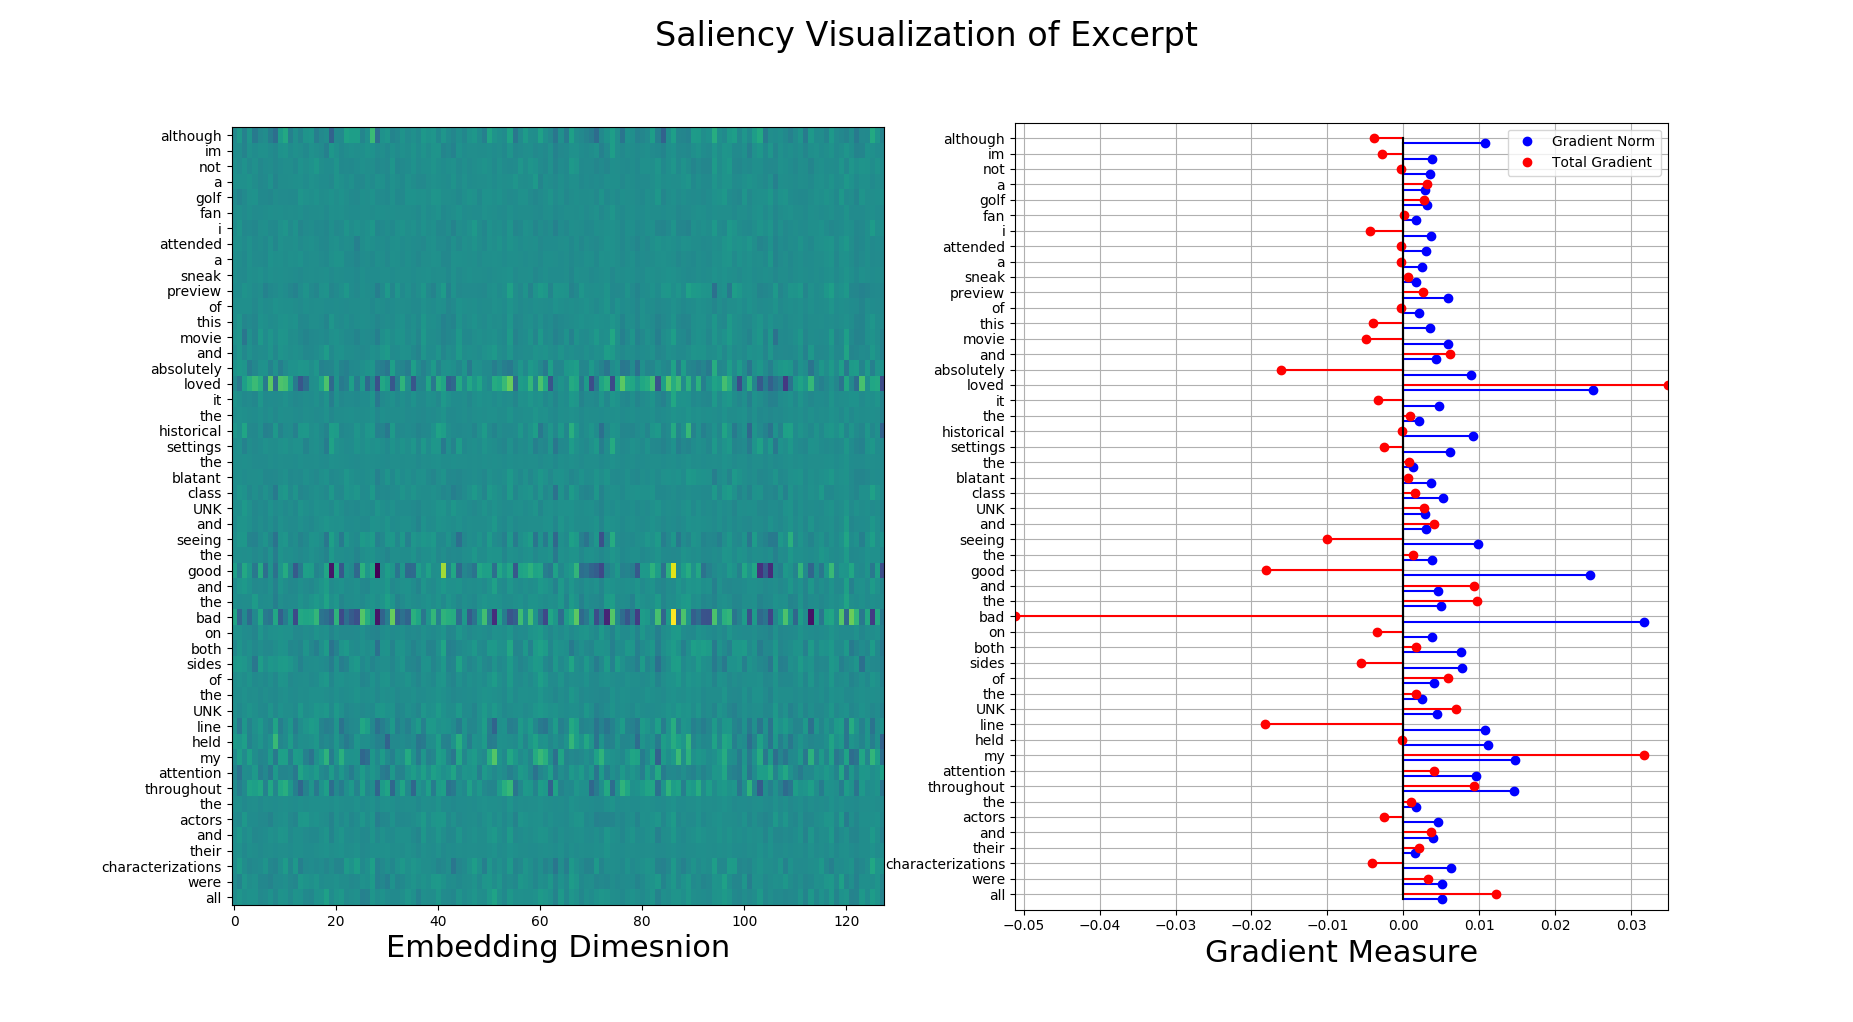
\includegraphics[width=\textwidth]{saliency.png}
    \caption{Different measures of word sentiment/importance}
    \label{fig:saliency}
\end{figure}

In our word embedding, the average value of $\mu$ was $-0.017$, but there was significant variation across embedding dimension.  The average standard deviation was fairly constant over embedding dimension, with a value of $0.55$.  The exact value of the result is not important however.  What this tells us is that words associated with larger gradient norms have a proportionally larger chance of producing an outlier, at least according to the linear approximation.

